\makeatletter
\def\input@path{{../}}
\makeatother
\documentclass[../main.tex]{subfiles}
\chapter{Atoms}
\graphicspath{
  {"../assets/images/"}
  {"../../assets/images/"}
}
\section{What is an atom?}
If we take anything physical in our world, and start tearing it down into
smaller and smaller chunks, eventually we end up looking at a structure we call
an "atom". For a long time, humans resisted the idea that there was such a
gadget, today, we put a lot of energy into researching what happens if we tear
and atom apart to see what it is made up of. We even want to go a bit further and
see what those atomic parts are made up of.

Welcome to the world of high-tech physics!

We will not dive smaller than the basic atom. (Real, serious physicists are
trying to go much farther!) That will let us look at its most basic parts.

Some of this, you should have learned in your high school chemistry class!

\subsection{Basic Atom Structure}
An atom is sort of like a tiny solar system. There is something big in the
center of this system, and a bunch of smaller things flying around that center
in tiny orbits.
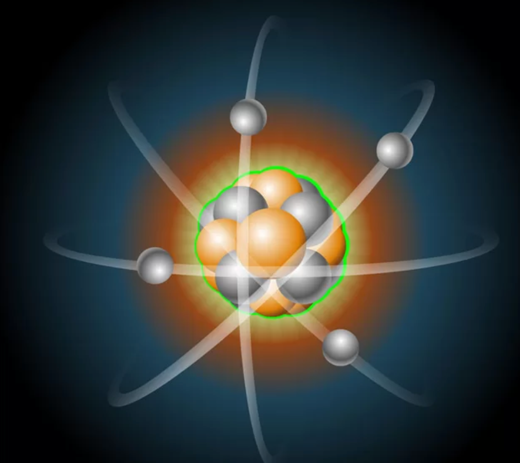
\includegraphics{atomic-structure.png}[H]

Atoms are pretty small. Estimates as to their size depends on the material, but
a single atom is as small as :math:`10^{-8}cm` in size. That is pretty small.
But, amazing as it might seem, we can build machines that can move single
atoms. Take a look at this image, created by IBM engineers in 1989. The image
was taken using a scanning electronic microscope!

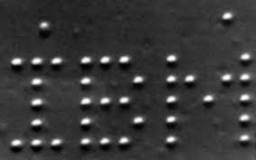
\includegraphics{IBMlogo.jpg}[H]

Those bumps are actually single atoms, nudged into place to create this logo.
Amazing!

\subsubsection{Electrons}

The particles flying around the center are ``electrons``. These particles are
tiny! Linus Pauling, a Chemist who won the Nobel Prize for Chemistry in 1954,
thought they were on the order of :math:`< 10^{-18}cm` in size. That is pretty
small.

These electrons carry a ``charge`` (actually a negative ``charge``). 

..  note::

    Contrary to popular thinking, if something is positively ``charged``, that
    means it has fewer ``electrons`` than it wants to have. If something is
    negatively ``charged`` it has too many ``electrons`` than it wants to have.
    ``Electrons`` are attracted to positively ``charged`` things, and repelled
    by other negatively ``charged`` things.

    So, two ``electrons`` hate each other, and want to keep away from each
    other.

\subsubsection{Protons}

At the center of our tiny solar system sits a clump called the ``core``. This
``core`` is made up of two more tiny elementary particles. One is the
``proton``.

``Protons``, are about :math:`10^{-13}` meters in size. That is
(1000 times bigger than an ``electron``!)

```Protons`` carry a positive ``charge``. In a single atom, there should be as
many ``protons`` as there are ``electrons`` flying around this atomic core. 

As long as this is true, the atom is happy, and the electrons sit there, flying
around the core with its pile of ``protons``.

\subsubsection{Neutrons}

The second particle in the ``core`` is called a ``neutron``, which carries no
charge. ``Neutrons`` are about the same size as ``protons``. ``Neutrons`` are
not attracted to either ``electrons`` or ``protons```. They just sit there,
stuck to the ``protons`` in that core. What they do is give the atom addition
mass (think weight).

\section{Atomic Numbers}

We like to classify things. At the level of atoms, we assign an ``atomic
number`` to each kind of atom we discover. Those ``protons`` and ``neutrons``
in the ``core``` both act in a similar way. So we lump them together and call
then ``neucleons``. The ``atomic number is the number of ``neucleons`` in the
atom. (Where do you think the term ``neuclear physics`` came from?)

\subsubsection{Ions}

Since ``electrons`` are always flying around, and the core just sits there,
there is the possibility that an electron will get close enough to another atom
that it will fly off of the first atom, and join in the mess of electrons
flying around the second atom. The atom that the ``electron`` left is now left
with more ``protons`` than ``electrons`` and has a net positive `charge``. It
is not happy in this state, but there is not much it can do. The second atom is
also "unbalanced". It has more ``electrons`` than ``protons`` and has a net
negative ```charge``. That second atom is also unhappy. We call these "unhappy"
atoms ``ions``. 

..  note::

    We have names for each kind of ``ion``. A positively charged ``ions`` is
    called an ``cation``, and a negatively charged ``ion`` is called an
    ``anion``. ``Cations`` are also called "metals", and an Anion` is called a
    "non-metal``. The terns ``anode`` and ``cathode`` refer to points in a
    device where the charge is more positive, or more negative. Makes sense,
    right?


We can create ``ions`` by heating atoms up and firing a stream of ``electrons``
at them. Those electrons can knock off other electrons from each atom, setting
up this ionized state. The mess at the middle of this action is called a
``plasma``, and it has interesting properties, but we will not explore them
here. Plasmas might be interesting if you need to wipe out space aliens!

\subsubsection{Stable Ions}

Some ``ions`` are content with being "unbalanced", but only up to some limit.

For example Sodium is an element with 11 ``protons`` in the core, and 11
``electrons`` spinning around. It is happy in this normal state. But, Sodium
will tolerate losing an electron, becoming a Sodium ion. The chemical symbol
for Sodium id **Na** and the term for the Sodium ion is :math::`Na^{+}`. This
ion is positively charged).

Chlorine is another element, this one with 17 ``protons``, and 17
``electrons``. Chlorine is happy to accept another electron, becoming a
Chloride ion. The chemical symbol for Chlorine is **Cl**. The Chloride ion is
:math:`Cl^{-}`. It is negatively charged.

When these two ions get near each other, they "bond". The electron does not
move from one to the other, but the attractive force causes them to move close
together.  This "bond" is pretty strong, and the result is a lattice of atoms we
call a ``crystal``. This one is known as "salt"! The chemical symbol for this
is **NaCl**. The original ions are still ions, but they are quite happy being
close together.

\subsubsection{Metals}

We already mentioned the term ``metal``. That term describes an element with a
strong willingness to lose an electron, becoming a ``cation``. When many of
these atoms get together in a material like copper, they collectively let
electrons fly off, forming a sea of electrons that fly around, seemingly at
random, surrounding the entire collection of atoms. These electrons are called
``free-electrons`` because they have no real home on any single atom. This sea
of electrons produces something called "conductivity", a willingness of a
material to let electrons "move" easily. New ``electrons`` can join into this
sea, others can be pulled off.

\section{Electric Fields}

An electric field is a region around an charged particle. The charge at any
point in that area around the charge is measured in something we call
``volts``. Voltage is a measure of the ``electrostatic potential`` energy
available at that point. Near a positive charge, the voltage is high, near a
negatively charged particle it is low. 

It takes energy to move a point from one voltage to another one. It takes a lot
of energy to move a voltage higher, just as it takes energy to lift an object
to a higher position above the ground. Once at the high point there is a
"potential" to release that energy by moving the object (or the charge) to a
lower point. 

The strength of this electric field is measured in something we call ``volts``.

When electrons move, they generate a magnetic field around them, often called
an ``electromagnetic field``, since there is a magnetic field and an electric
field at work at the same time. All of this is described by ``Maxwell's
Equations``, which are the foundation of many technical disciplines, especially
``radio``. Those waves propagate through space, interact with other metals, and
induce electrons to move in those metals. (Hey, that is how radio works!)

\subsection{Electricity}

We now have enough background to explain how electricity works (well at least
in a (very) simple way!)

I have a cool book called "There are no Electrons, Electronics for Earthlings" :cite:`Amdahl:1991`. In
that book the author describes electrons as "party animals" who need to party.
The parties are all at positively charged points. The electrons are attracted to
those parties, and work tirelessly to find their way to them! However, they
must travel over "conductive" paths. Something like a copper wire will do
nicely!

\subsubsection{Batteries}

There has to be a source of both positive and negative charges in any
electrical system. That source is often called a ``battery``. The battery is a
device that can hold both positive and negatively charged particles, but it
separates them with a wall, preventing them from getting together. Instead, the
battery has two terminals, One will let electrons loose, the other is where the
party is.

Now, if we provide a path from the electrons to the party, those electrons will
fly. Actually a stream of electrons will join the sea of free electrons in the
mtal, and that will cause many of them to seem to move toward the other end.
The path is called a "circuit".

..  warning::

    It is vitally important that we not allow all the electrons to the party at
    once. That can cause very harmful side effects, like smoke! That is called
    a "Short Circuit". Batteries have been known to explode if this happens!

    Usually, we put some gadget in the circuit that slows things down. A light
    bulb will do. The bulb is designed so that it slows the electrons down.
    They want to move, so they get hot. The heat produces light. Cool! (Well,
    actually, HOT!)


\section{Who Cares?}

This is a computer architecture course, What does this have to do with
Computers?

Well, think about this simple C++ code fragment:

\begin{listing}

int x, y=5;

x = y;
\end{listing}

What needs to happen to make this statement work? How do you think the
computer is going to make this actually happen? The answer is simple. It will
launch some of those party animals, and cause them to travel from the place
called "y" to the party at the place called x". We design a machine that
causes the electrons to carry "data" along as they move to the party!

Wow!

Now, don't panic. You do not need to understand all of the physics in this
discussion. It will not appear on a test. 

I, on the other hand, and one of those crazy folks who keeps digging, as far
down as I can go. It gets more fascinating as you dig deeper. 

..  warning::

    You can kill a lot of time Googling all of this! You have been warned!













